%******************************************************************
%******************************************************************
\chapter {Data Analysis Framework}
\label{data_preprocessing}
%******************************************************************
%******************************************************************

This chapter is dedicated to analysis of time-resolved X-ray data. It divides into two extensive sections: data enhancement (Section \ref{data_processing}) and further analysis of the computed optical flow results (Section \ref{data_analysis}).
 
In Section \ref{data_processing} we start the discussion of data pre-processing (or filtering) to correct image defects. This step always precedes any further data treatment and optical flow computation. We consider three topics which are of key importance: image noise filtering, brightness corrections and contrast adjustment.     

In Section \ref{data_analysis} we give a list of data analysis routines which we employ in the application section of the current work. These routines, together with a variety of optical flow methods constitute our framework for time-resolved data analysis. We distinguish five individual \textit{tasks}: analysis of the computed motion field; motion-based segmentation; detection of temporal changes which are not attributed to the motion itself; automated tracking and image registration/alignment.

%In Section \ref{visualization} we present and briefly discuss data visualization methods used in the scope of this work to depict the result of optical flow computation (i.e. the displacement field) and results of the further motion analysis.       
 

%--------------------------------------------------------
\section{Data Preprocessing}
\label{data_processing}
%--------------------------------------------------------

In this section we present a first step in our data treatment pipeline, namely data preprocessing. The purpose of this step is to correct various image defects that might be present due to  non-optimal experimental conditions, physical properties of the process, imprecise detector system, or  artificial errors introduced by an image reconstruction procedure. Such image defects might deteriorate the result of data analysis and thus should be corrected before any further optical flow computation or analysis steps are undertaken.

We assume that data which is provided for the image processing already represents the best possible quality which can be achieved by the data acquisition process. Otherwise, the experimental conditions should be readjusted and optimized. However, this is not always possible and frequently the image acquisition system is employed to its technical limits. 

As an example, image noise affects the ability to detect small feature details, especially for the low contrast data - when brightness level differs only slightly for separate image features. To increase signal-to-noise ratio and, thus, to improve data quality, it is necessary to increase the number of detected photons. This can be done by increasing the beam intensity, increasing the exposure time or acquiring and averaging several image frames. All of this, however, will lead to a higher dose deposition, which can affect the viability of the specimen in the case of biological applications. Another option is to increase the pixel size by combining several neighbor pixels, which will allow to detect more photons, resulting in a higher signal-to-noise ratio. But, in this case, the improvement in signal-to-noise ratio is obtained at the expense of poorer spatial resolution. This illustrates a fundamental trade-off between image quality and dose deposition. Moreover, there is also a trade-off between individual parameters of image quality, i.e. spatial resolution, features contrast and noise. Furthermore, the optimization of experimental setup could be time consuming and, given the limited time for experiments on a synchrotron, dealing with image data as a post-processing step could be more practical. That is why it is reasonable to sacrifices the image quality for the ability to capture physical characteristics of dynamical process, and then utilize data processing as a correction step. 

It is important to emphasize, that by the term \textit{data preprocessing} we assume both data restoration (correction) and data enhancement. However, both procedures are not the same and serve different purposes. Unlike data enhancement, which is a subjective routine and aimed on improving visual appearance of certain image details or features, image restoration is based on mathematically justified image correction. There might be cases when the same image processing procedure serves both purposes. For example, correcting image brightness variations could improve visual analysis of image sequences, since image flickering could be distracting and obscure important changes. On the other hand, it could also correct pixel data for the use of certain optical flow models (e.g. grey value constancy assumption).



 


\subsection{Noise Filtering}
\label{noise_filtering}

\textit{Image noise} is the unwanted fluctuations of the pixel brightness in an image. This results in a degradation of image quality and deteriorates data analysis.  The noise which is generated within an imaging system is usually a combination of a number of independent noise
sources. In general, it is not possible to identify, and thus to filter individual noise contributions separately. To quantify image variations due to the noise, a scene in which the resulting image is expected to have a uniform brightness might be used. Then, a noise content of the image (noise power $P_n$) is given by the variance, i.e. the square of the standard deviation, of the pixel grey values in local image region. To estimate the noise influence one should compare it with the average amount of intensity in the same region (signal power $P_s$).  The \textit{signal-to-noise} ratio (SNR) is the ratio of the intensity of the signal (pixel brightness) to the noise power $SNR = \frac{P_s}{P_n}$. However, in cases when noise properties cannot be described as random or having \textit{normal} statistical distribution, it is more difficult to estimate the amount of noise. 

In the following sections we shortly describe a number of \textit{noise models} which are the most relevant for the processing of X-ray images and optical flow analysis. Then we provide correction techniques (noise filters) which allow us to reduce the amount of noise and to recover useful information. This, in turn, will improve the results of optical flow computation.   




\subsubsection{Noise Models}
\label{noise_models}

The common sources of noise in images taken with X-ray imaging systems are photon noise, which originates due to the discrete nature of X-ray radiation (and electromagnetic radiation in general) and interaction of X-ray with matter, and electronic noise from the digital detector systems. Additionally, the process of digitization also adds noise (quantization noise), but we assume that this type of noise does not contribute much to the overall noise level.
\\
\\
\textbf{Gaussian noise}
\\
A popular noise model which is considered in various fields of Signal Processing and Computer Vision is \textit{Gaussian noise}. It has a probability density function (or normalized histogram), which is given by:
$$G(x,\mu, \sigma)= \frac{1}{\sigma \sqrt{2 \pi}} e^{-\frac{(x-\mu)^2}{2\sigma^2}}, $$
where $x$ is the pixel brightness, $\mu$ is the mean brightness value and $\sigma$ is its standard deviation.
This model is a very convenient from the mathematical point of view and simulates many real world random (stochastic) processes. That is why it is widely used in image processing to contaminate images with noise.  However, this model does not adequately represent physical properties of image acquisition process in most medical systems, including X-ray imaging, where an image has a spatial and temporal randomness characterized by Poisson statistics. 

In the current work we decide to keep this noise model for the sake of having a systematic experimental approach and direct comparability with the literature on optical flow. We start all the experiment on noisy images with this simple model and then proceed with the more suitable ones such as photon and impulse noise models. 
\\
\\
\textbf{Photon noise}
\\
\textit{Photon noise} (also known as quantum noise or shot noise) arises from the statistical properties of electromagnetic radiation - an imaging sensor receives within a time interval of $\Delta t$ (exposure time) on average $N$ electrons by absorption of photons. The average rate of received photons per unit time $\lambda$ is given by $\lambda = \frac{N}{\Delta t}.$  During each exposure a different number of photons are registered by the detector element. A random process in which an average $\lambda \Delta t$ events are counted is described by a Poisson distribution $P(\lambda \Delta t)$:
$$ P(\lambda \Delta t) = \frac{(\lambda \Delta t)^n}{!n}  e^{- \lambda \Delta t}, n \geq 0,$$
with the mean and variance: $\mu = \lambda \Delta t $ and $\sigma^2 = \lambda \Delta t$ respectively.  An important property of a random process according to Poisson distribution is that it is not independent of a signal and is not additive. Additionally, the signal-to-noise ratio increases as an average brightness level gets larger, which means that the more x-ray photons are detected, the higher the signal-to-noise is and the less noise is contained in the image data. The
photon noise is a fundamental and unavoidable source of noise in medical imaging. For an efficient and optimized imaging system it is the dominant source of random fluctuation in image data \cite{Dougherty09}.

An important contribution of our work is that in addition to a classical Gaussian noise model we include an extensive discussion of performance of optical flow methods on a physically justified noise model such as photon noise.
\\
\\
\textbf{Spike noise}
\\
Another type of noise which could be useful to consider for our class of applications is so-called \textit{impulse noise} (also salt-and-pepper or \textit{Spike} noise). This type of noise is usually caused be the errors in data transmission or damaged sensor elements  of the digital detector system ("dead" or saturated pixels).  The strength of the corruption by impulse noise is usually of much more influence compared to other types of noise, since such type of noise is recorded as an extreme values, so they are equal or close to the maximum and minimum values of dynamic range of an image.
This type of noise is usually quantified by the percentage of pixels which are corrupted.

Despite the fact, that sometimes it is possible to correct such corrupted pixels using the dark field correction (which will be described later in Section \ref{flat_field_correction}), we choose to include this type of noise in our experiments on noise. We consider this type of noise as very helpful to evaluate  the performance of optical flow methods and data correction techniques with respect to data outliers.
   


\subsubsection{Noise Filters}
\label{noise_filters}
         
In the previous section we introduced several noise models which we will use for our experiments on noisy data (Sections \ref{exp_noise} and \ref{experiment_noise_reduction}). Here we present methods to restore image details from the noisy images, with the aim to possibly improve results of optical flow computation. There is a tremendous amount of literature on image denoising methods. For this work we limit our experiments only on those methods which are widely available, easy to implement and are well understood from the mathematical point of view. Here we do not aim to fully cover this topic. For in-depth information on denoising methods the reader is referred to the extensive literature. To enhance image data with respect to noise we consider four filters: Gaussian filter, bilateral filter, median filter, anisotropic diffusion filter.

An important assumption for any denoising method is that the pixel size (resolution) is much smaller then the important details which we aim to recover.  
\\ 
\\
\textbf{Gaussian Filter}

A commonly used approach to filter noise is a \textit{Gaussian smoothing}. 
It can be implemented as a convolution of the image with the Gaussian function. This  filter reduces noise  from the image, however, it also blurs image edges and reduces image contrast.   It can introduce other artifacts such as merging of nearby structures. Moreover, the data outliers are not completely filtered, but only averaged in a local neighborhood, which means that the corrupted pixel data could be spatially extended. Note, that Gaussian smoothing corresponds to the linear isotropic diffusion process. The implementation of Gaussian low-pass filtering is done via computing a weighted average of pixel values in the neighborhood, with the
weights decreasing with the distance from the neighborhood center.
\\ 
\\
\textbf{Bilateral Filter}

\textit{Bilateral filtering} removes the noise while preserving image
edge information, which is done by a weighted average of intensity values from nearby pixels.
An important property of the bilateral filter, is that the weights depend on both geometrical closeness of the pixels and their photometric differences (e.g. grey values) \cite{Tomasi98}.

The filtering procedure can be expressed in the following way:
$$I_{bilateral}(\textbf{x}) = \frac{1}{W_p} \sum_{\textbf{x}_i \in \Omega} I(\textbf{x}_i) f_r(|I(\textbf{x}_i) - I(\textbf{x})|) g_r(|\textbf{x}_i - \textbf{x}|),$$
where the normalization factor is:
$$W_p = \sum_{\textbf{x}_i \in \Omega} f_r(|I(\textbf{x}_i) - I(\textbf{x})|) g_r(|\textbf{x}_i - \textbf{x}|),$$
where $I$ is the original image, $x$ is the coordinate of the current pixel being processed; $\Omega$ is the spatial window mask centered at location $x$; $f_r$ is the range kernel to filter differences in pixel brightness; $g_s$ is the spatial kernel to filter differences in geometrical distances. 

Among the advantages of the bilateral filter are simple implementation and non-iterative nature of the algorithm.
\\
\\
\textbf{Rank Filters}

A drawback of smoothing or averaging filters is that they produce undesirable blurring on object boundaries, which are represented by image edges. A possible solution to this problem is to discriminate pixel values by ranking them in a local neighborhood. A common choice is a \textit{median filter} which selects the median value in the ordered list of grey values and uses this value as a new result for the central pixel.  
Median filter provides excellent performance for certain types of noise, especially impulse noise, which was discussed in the previous section. If a pixel contains an extreme brightness value ("dead" or saturated pixel), it is substituted by an acceptable value from a local neighborhood.
The important property of the median filtering is that is an \textit{edge-preserving filter}. However, for very large neighborhood sizes small image details could be completely eliminated.  

To implement a median filtering one may choose between different  sizes and shapes of the neighborhood. Several mask patterns are possible: a 4-nearest neighbor cross, a ($3 \times 3 $) square,  a ($5 \times 5 $) circular, etc. This different neighborhood patters are shown in Figure \ref{fig:median_mask}. Typically, a square mask is easier to implement, however, as the mask size increases the use of a pattern which approximates a circular region is important to produce more isotropic filtering \cite{Russ11}. For implementation of median filtering in the current work we opt to use a circular median filtering mask. 


\begin{figure*}[ht]
  \centerline{
    \mbox{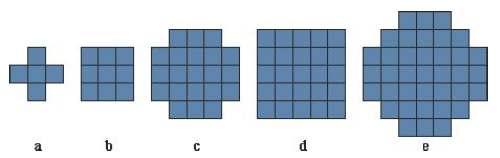
\includegraphics[scale=0.55]{figures/median_mask.png}}
  }
  \caption[]{Shapes of 2D neighborhood mask for median filtering. \textbf{(a)} 4-nearest neighbor cross. \textbf{(b)} a ($3 \times 3 $) square. \textbf{(c)} ($5 \times 5 $) circular. \textbf{(d)} ($5 \times 5 $) square. \textbf{(e)} ($7 \times 7 $) circular. Image: \cite{Russ11}.}
  \label{fig:median_mask}
\end{figure*}

Another useful approach is to consider a more sophisticated ranking of neighborhood information. This step is driven by the fact, that median filter removes small details which are twice smaller then the size of the median mask and also removes sharp corner details. A special case of corner-reserving median filter, is a \textit{hybrid median filter} \cite{Nieminen87, Russ11}. This filter ranks all the pixels in different sets. In the first group there are 4 nearest neighbours forming a "+" sign and the second group are pixels which are located in diagonal locations with respect to the central pixel (forming a "x" sign). Then, median values from these two sets are compared with the central pixel. The idea is sketched in  Figure \ref{fig:hybrid_median_filter}.
\begin{figure*}[ht]
  \centerline{
    \mbox{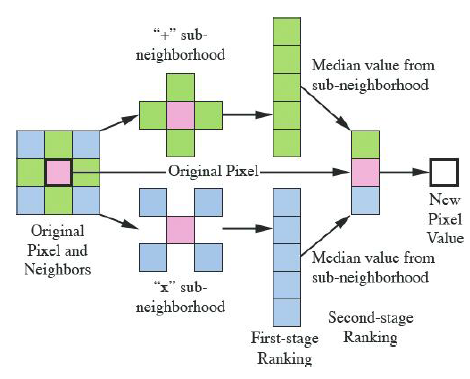
\includegraphics[scale=0.65]{figures/hybrid_median_filter.png}}
  }
  \caption[]{A sketch of hybrid median filter, which preserve corners and small coherent structures. Image: \cite{Russ11}}
  \label{fig:hybrid_median_filter}
\end{figure*}
\\
\\
\textbf{Anisotropic Diffusion}

\textit{Anisotropic diffusion} (also known as Perona - Malik diffusion \cite{Perona90}) is a method which aims to reduce image noise without removing image edges representing an important features. Additionally, such types of filters can posses even edge-enhancing properties \cite{Weickert98}. The smoothing is done by means of a diffusion process in which the strength of the diffusion is controlled by derivatives of the image brightness values.
Anisotropic diffusion is define as:
$$ \frac{\partial I}{\partial t} = \text{div} ( c(x,y,t) \nabla I),$$
where $I(x,y,t)$ is an image in a domain $ \Omega_{2} \subset \mathbb{R}^2$, $\nabla$ denotes gradient operator, div() is a divergence operator, $c(x,y,t)$ function controls the rate of diffusion depending on image data at pixel location $(x,y)$.
In a seminal paper of Perona and Malik the diffusivity $c(x,y,t)$ are:
$$c(|\nabla I|) = e^{-(|\nabla I| / \epsilon)}$$
or
$$c(|\nabla I|) = \frac{1}{1 + (\frac{|\nabla I|}{\epsilon})}$$
where $|\nabla I|$ is a magnitude of the image gradients and $\epsilon$ is constant which is choose experimentally or depending on a noise scale.

Anisotroipic diffusion is a flexible and highly adjustable filter. With different parameters one my obtain a very distinctive filtering results. However, what might be an advantage to produce better results, also can be a drawback, since it is not easy to optimize numerous parameters to get the best possible result. Additionally, the implementation is not trivial and the filter is computationally demanding (being an iterative method). 

Carefully weighting all pros and cons we use this filter for our quantitative comparison of denosing filters, since anisotropic diffusion is a powerful and flexible method, with many degrees of freedom. 

We use an implementation based on the paper of \cite{Tschumperle05}. A freely available implementation can be access via a web link: \\
\url{http://rsb.info.nih.gov/ij/plugins/anisotropic-diffusion-2d.html}.  

%-------------------------------
% Temporally excluded
%-------------------------------
%\\
%\\
%\textbf{Non-Local Means}
%\todo{Include or exclude from thesis}



\newcommand{\imageSize}{0.65}

\begin{figure*}[!ht]
  \centerline{
    \mbox{\includegraphicslabeledw[scale= \imageSize]{figures/noise_rub1_original_crop.png}{a}}
    \mbox{\includegraphicslabeledw[scale= \imageSize]{figures/noise_rub1_sigma_2p0_crop.png}{b}}
  }
  \vspace{3pt}
  \centerline{
    \mbox{\includegraphicslabeledw[scale= \imageSize]{figures/noise_gauss_2p0_crop.png}{c}}
    \mbox{\includegraphicslabeledw[scale= \imageSize]{figures/noise_median_3p0_crop.png}{d}}
  }
  \vspace{3pt}
  \centerline{
    \mbox{\includegraphicslabeledw[scale= \imageSize]{figures/noise_bilateral-5p0-70_crop.png}{e}}
    \mbox{\includegraphicslabeledw[scale= \imageSize]{figures/noise_anisotropic-iter20_a1_0p5_a2_0p9_dt_20_edge_15_crop.png}{f}}
  }
  \caption[Noise filterst]{Performance of noise filters on \rub dataset with Gaussian noise with $n_{\sigma}$=10. \textbf{(a)} First frame of original image. \textbf{(b)} With Gaussian noise with $n_{\sigma}$=10 added.  \textbf{(c)} Gaussian smoothing filter. \textbf{(d)} Median filter. \textbf{(e)} Bilateral filter. \textbf{(f)} Anisotropic diffusion filter.}
  \label{fig:noise_filters}
\end{figure*}
\vspace{7pt}

\noindent Comparison of different noise filtering methods is presented in Figure \ref{fig:noise_filters}.

                 
\subsection{Brightness Correction}
\label{brightness_correction}


The most commonly used assumption in image analysis to identify or compare pixel values is that the region representing the same object or feature should have the brightness value. However, in practice for real-world imaging scenarios such strict conditions could not always be fulfilled. 

For X-ray imaging the constancy and uniformity of the background brightness distribution can be affected because of various reasons, such as non-uniform beam profile due to spatio-temporal fluctuations of a light source, etc.  
Usually such effects can be corrected by recording a background image (without an object in the field of view) and then removing non-constant brightness variation (see Section \ref{flat_field_correction}). Depending on the image content, this can be implemented as a subtraction or division operation with a background and the image with an object. However, this procedure is not always feasible, especially for \textit{in-situ} or \textit{in-vivo} experiments, when one acquires a continuous sequence of images and brightness variations occur during the recording time. For this case we propose a proper brightness correction procedure. Here we describe the most popular methods to achieve this and later evaluate how different correction procedures influence the accuracy of optical flow estimation (see Section \ref{experiment_nonuniform_brightness}).          


\subsubsection{Illumination Models}
\label{illumination_models}

As we outlined previously, background brightness distribution can be non-constant over time or non-uniform spatially for a sequence of X-ray images. This property of X-ray data is of crucial importance for the choice of appropriate data constancy assumptions for the design of optical flow models (see Section \ref{data_constancy_assumptions}). In the literature on optical flow methods this problem is referred to as "changing illumination conditions". 

To correctly model optical flow assumptions it is important to consider realistic illumination scenarios. Two important models in the literature on the optical flow are: \textit{additive} illumination and \textit{multiplicative} illumination \cite{Weijer04, Mileva07}. Additionally, one may distinguish between \textit{global} and spatially \textit{local} changes.
In Section \ref{data_constancy_assumptions} on the available data terms  we already discussed that the gradient constancy assumption is invariant under global additive illumination changes, however it is not suited for the case if there is also a multiplicative part.

It is important to note, that increasing an exposure time while recording an X-ray image corresponds to global multiplicative brightness changes. Thus, to apply optical flow methods, an appropriate choice of the data term which is robust under this type of brightness changes is an crucial aspect. This will be discussed in the experimental section \ref{exp_data_terms_brighntness}.

Typically, to tackle with varying brightness conditions optical flow methods make use of different photometric invariants derived from color models \cite{Mileva07, HarmonyFlow}. Such transformations are invariant under general illumination changes.  
However, since color information is not available for X-ray images we are enforced to search for another reliable solutions, which we present in the following sections. 

        

        
\subsubsection{Flat-field Correction}
\label{flat_field_correction}

The simplest approach to correct background non-uniformities is to perform so-called \textit{flat-field correction}. In this case a "flat" image, without an object in the field of view is recorded. Then this image is used to eliminate the brightness pattern from the image with a specimen. In a general form the flat-field correction can be computed as:
$$I_{filt} = \frac{I_{raw} -  I_{dark} }{I_{flat} - I_{dark}},$$
where $I_{raw}$ is a recorded raw image, which has to be corrected, $I_{flat}$ is a flat-field image and $I_{dark}$ is a dark-field image. The dark-field image is an image captured with no illumination. In other words, it is an image of the sensor noise. An average of several dark-field frames provides a possibility to correct for the fixed-pattern noise, including dark ("dead") and saturated ("hot") pixels. 
For the case of X-ray data, since the recorded images represent the absorption of a sample according to the Beer's law (for the case when absorption is dominating the image contrast) we may also perform a logarithm transformation to recover the physical thickness of structures:
$$I_{filt} = \frac{\text{log}(I_{raw} -  I_{dark}) }{\text{log}(I_{flat} - I_{dark})}$$

However, as we mentioned before, a flat-field correction is not always possible for \textit{in-situ} or \textit{in-vivo} experiments.      

\subsubsection{Fitting Background}

One approach to eliminate uneven background from the recorded image, without a flat-field image available is to measure an overall brightness in different parts of the image and then interpolate the result. Then the obtained brightness pattern might be used for image correction. A good choice for the interpolation function is a polynomial interpolation, which gives good results for relatively gradual brightness variations. Another choice is to perform least-squares fitting of sample points distributed over the image domain. The distribution of sample points could be automated (for example using a grid or object detection) or manual.  

\subsubsection{Image Leveling}
\label{image_leveling}

In the case when the background changes more irregularly, so the fitting of a simple function cannot be performed, a different approach might be useful. For this method one assumes that the image features have smaller size then the scale of brightness variations.
The background image is estimated by applying an averaging or ranking filter with a large spatial mask. Than, this background image is subtracted from the original image frame to remove brightness variations.

In the current work we employ two types of filters, namely Gaussian smoothing filter and median filter (See Section \ref{noise_filters}). Important parameters for such a filter are the shape and the size of a spatial mask.  One should note that brightness variations can be one-dimensional (e.g. horizontal stripes patters), in this case the filter can be implemented as a 1D stencil. Figure \ref{fig:image_leveling} shows the application of image leveling methods to correct uneven brightness patterns.

\begin{figure*}[ht]
  \centerline{
    \mbox{\includegraphicslabeledw[scale= 0.38]{figures/contrast_adjust_orig.png}{a}}
    \hspace{3pt}
    \mbox{\includegraphicslabeledw[scale= 0.38]{figures/contrast_adjust_corr.png}{b}}
  }
  \caption[Noise filterst]{Non-uniform background correction using image leveling with the Gaussian smoothing filter with a spatial mask $\sigma=15$. \textbf{(a)} Original image. \textbf{(b)} Corrected image. }
  \label{fig:image_leveling}
\end{figure*}




\subsubsection{Log Transform}

Another approach to deal with local brightness variations (including additive and multiplicative intensity changes) is to use a so-called log-derivatives \cite{Mileva07}.
In this case the original image grey values are transformed into a logarithmic scale, then gradients of these log-derivatives are considered as constancy assumptions for the computation of optical flow. Such transformation is more robust under multiplicative intensity changes.

We evaluate this approach in the experimental Section \ref{exp_data_terms_brighntness}, where we check the performance of different data terms for changing brightness conditions. 




\subsection{Contrast Adjustment}
\label{contrast_adjustment}

The range of brightness values represented on the image is known as the \textit{dynamic range}. It can be measured as a difference between maximum and minimum values. Ideally, the dynamic range obtained by the interaction of the radiation with the sample - for the case of X-ray imaging - should coincide with the available  dynamic range of the detector system. In a case if it is wider than the one of the detector, the image histogram is cutted. The brightness values which fall inside this cutted regions are inevitably lost. Additionally, extreme pixel values which corrupt the range of histogram can be caused by data outliers, such as "dead" or "hot pixels" and can be corrected as a preprocessing step to improve the visibility of image details.

An image property which is related to the dynamic range is a \textit{contrast}. In the case when the dynamic range of an image covers all brightness values produced by the imaging system (including interaction of X-rays with a sample), the image exhibits high contrast. On contrary, when dynamic range is low (only a narrow range of similar grey values present in the image), the image has a low contrast. 
It is important to note, that the dynamic range and image contrast are related, but not identical concepts. For instance, images with bimodal histogram (peaks on the lower and upper parts of the histogram) exhibit higher contrast than images with smooth, even histogram.  For the ideal imaging session one is interested to both cover the full dynamic range of the image and provide maximum feature contrast.    

Since for optical flow methods the pixel grey values are the source of information to solve a correspondence problem, one may try to correct the image contrast not only to enhance the visibility of image details, but also to improve results of optical flow computation. In this section we present a number of techniques to achieve that and in Section \ref{experiment_local_contrast} we evaluate the influence of these methods on the accuracy of optical flow.    



\subsubsection{Contrast Estimation}
\label{contrast_estimation}

In Section \ref{noise_filtering} we discussed an important characteristic of the image, which is a signal-to-noise-ratio (SNR). Here we emphasize that for the analysis of X-ray images (and medical image in general) a concept which is even more important is a \textit{contrast-to-noise ratio} (CNR):
$$C = \frac{|S_1 - S_2|}{\sigma},$$
where $S_1, S_2$ are the brightness of structures in the region of interest and $\sigma$ is the standard deviation of image noise.  
For medical imaging applications the goal is to distinguish between different structures or between an object and a background. For this case the contrast-to-noise ratio is more descriptive and useful measure, since it relates both image noise and image contrast.  


\subsubsection{Contrast Enhancement}
\label{contrast_enhancement}

A frequent situation, especially for X-ray imaging with low exposure conditions, is when the images do not have the brightness range that covers the full dynamic range available for a detector system. On Figure \ref{fig:histogram_stretch} brightness values on the light and dark ends of the histogram are not used.
Expanding the brightness value to cover the full dynamic range may improve the visibility of local image features. This can be implemented with the linear brightness values mapping \cite{Gonzalez08}. This operation is often called the \textit{histogram stretching}. The result of this transformation is shown in Figure \ref{fig:histogram_stretch}b.

\begin{figure*}[ht]
  \centerline{
        \mbox{\includegraphicslabeledw[scale= 0.27]{figures/egg1.png}{a}}
        \mbox{\includegraphicslabeledw[scale= 0.27]{figures/egg2.png}{b}}
  }
  \vspace{3pt}
    \centerline{
    	\mbox{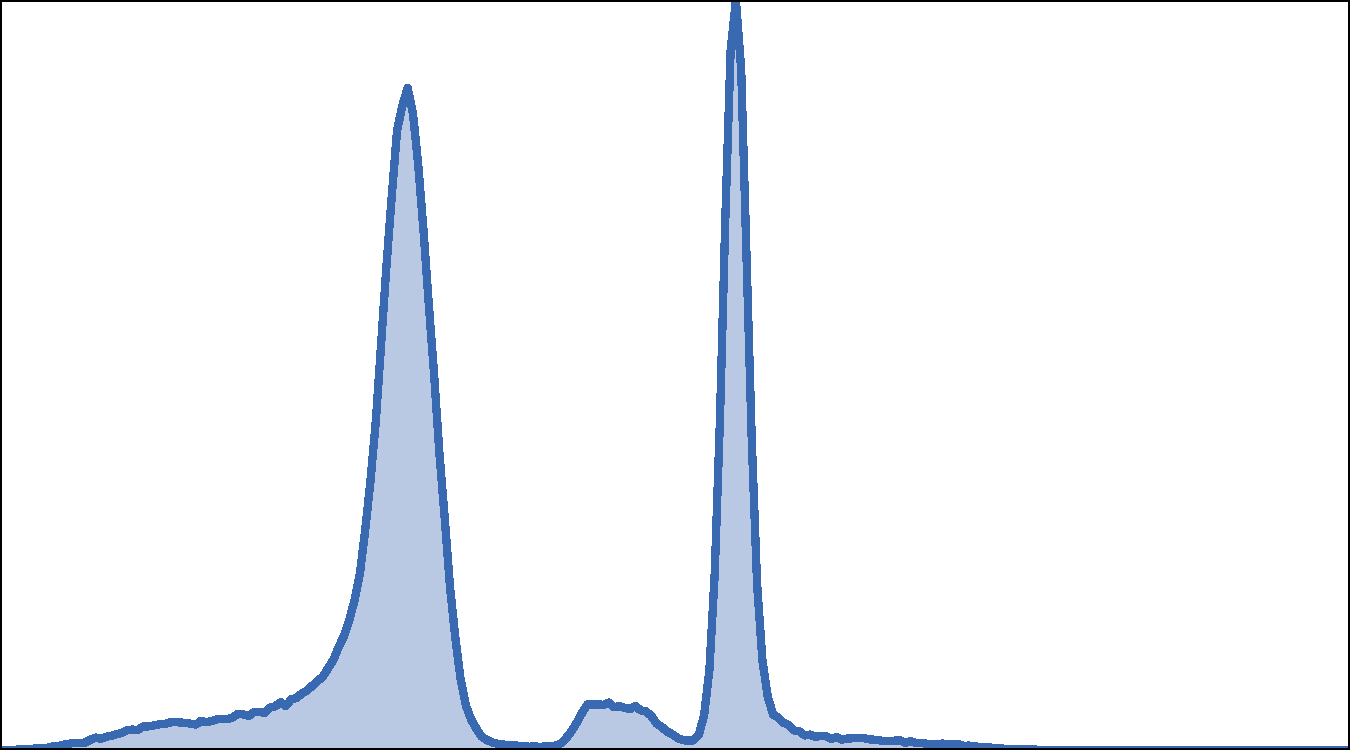
\includegraphics[scale= 0.29]{figures/egg1_hist.pdf}}
    	\mbox{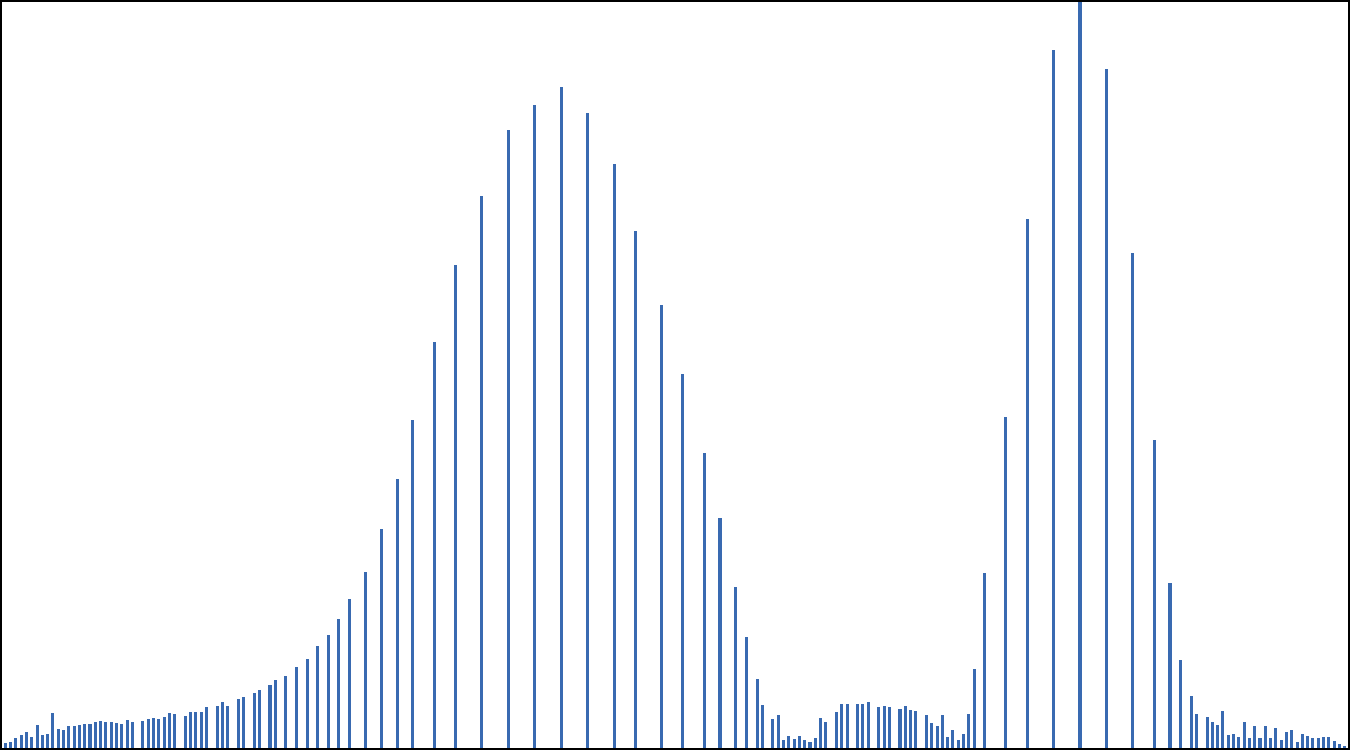
\includegraphics[scale= 0.29]{figures/egg2_hist.pdf}}
    }

  \caption[]{Example of a histogram stretching to improve the visibility of local image features. \textbf{(a)} Original radiograph with poor contrast. \textbf{(b)} Radiograph corrected using histogram stretching.}
  \label{fig:histogram_stretch}
\end{figure*}

In some cases the majority of pixel values occupy a narrow range of a histogram, but a few number of outliers represent extreme values (e.g. hot and dead pixels). In this case the histogram stretching cannot be performed, since the whole histogram range is used. This results in an ineffective use of dynamical range. One way to solve this, is to filter these outliers, e.g. using median filtering. However, this procedure also affects the pixel values in the correct range of brightness range. Alternatively, it is possible to dismiss a certain percentage of pixels on the histogram ends. As a result, these pixels will be saturated with minimum and maximum values, but the rest of histogram range will be used effectively. 

Note, that the aforementioned procedure is global and linear. To improve local visibility of image features, one may perform nonlinear, \textit{local contrast enhancement} \cite{Pizer87}. This technique perform brightness stretching based on a histogram of a local image region.    



%\subsection{[OPTIONAL] Image Decomposition}
%
%\comment{Find further information}

%\subsubsection{OPTIONAL: Edge Enhancement}

%\comment{Check!}


%--------------------------------------------------------
\section{Analysis Based on Optical Flow}
\label{data_analysis}
%--------------------------------------------------------



This section is devoted to an overview of data analysis methods, which can be applied after the optical flow results are computed. By further analysis of the obtained motion field one can extract a vast amount of quantitative information about dynamical processes. Although, several techniques can be closely related, in our \textit{data analysis framework} we identify four separate topics:
\begin{itemize}
	\item Motion / flow analysis 
	\item Motion-based segmentation
	\item Object tracking
	\item Image registration and alignment
	
\end{itemize}
In the following sections we describe in details each of these analysis methods.
   

%--------------------------------------------------------
\subsection{Motion Analysis}
\label{motion_analysis}
%--------------------------------------------------------
            
In this section we present a common techniques to analyze the motion field after the optical flow is computed.  The aim of these methods is to provide quantitative information about dynamical process. 
All of the presented methods are available in our data analysis framework. 

We define a \textit{vector field}  as a map $\textbf{F}: \textbf{R}^n \mapsto \textbf{R}^n $ that assigns each coordinate $\textbf{x}$ a vector $\textbf{F}(\textbf{x})$. 
A vector $\textbf{F}$ in an $n$-dimensional Euclidean space can be defined as an ordered list of $n$ real numbers  $\textbf{F} = \lbrace x_1, x_2, \ldots, x_n \rbrace$.
 
            
\subsubsection{Magnitude}
\label{magnitude}

An important property of a vector is its \textit{magnitude} or length (also referred as velocity). It is commonly defined as a Euclidean norm:
$$| \textbf{F} | = \sqrt{x_1^2 + x_2^2 + \cdots + x_n^2 } $$

Magnitude of the vector field is a useful measure to quantitatively describe physical characteristics of the dynamical process, distinguish between different moving object and analyze the velocity changes over time. 
To compute the magnitude of the flow field one might be interested to distinguish 4 scales:
\begin{itemize}
  \item Magnitude of an individual pixel at the location $\textbf{x}$
  \item Average magnitude within a particular object $O$
  \item Average magnitude inside a certain region of interest (ROI)
  \item Average magnitude for the entire image frame $I(\textbf{x})$
\end{itemize}
    

\subsubsection{Divergence}
\label{divergence}

\textit{Divergence} is a vector operator that measures as a single scalar value to which extent a vector field behaves as a sink or source at a given point. It can be defined for a continuously differentiable vector field $\textbf{F}=(F_x,F_y,F_z)$ as follows:
$$\text{div} \, \textbf{F} = \nabla \cdot \textbf{F} = \frac{\partial F_x}{\partial x} + \frac{\partial F_y}{\partial y} + \frac{\partial F_z}{\partial z} $$


\begin{figure*}[ht]
  \centerline{
    \mbox{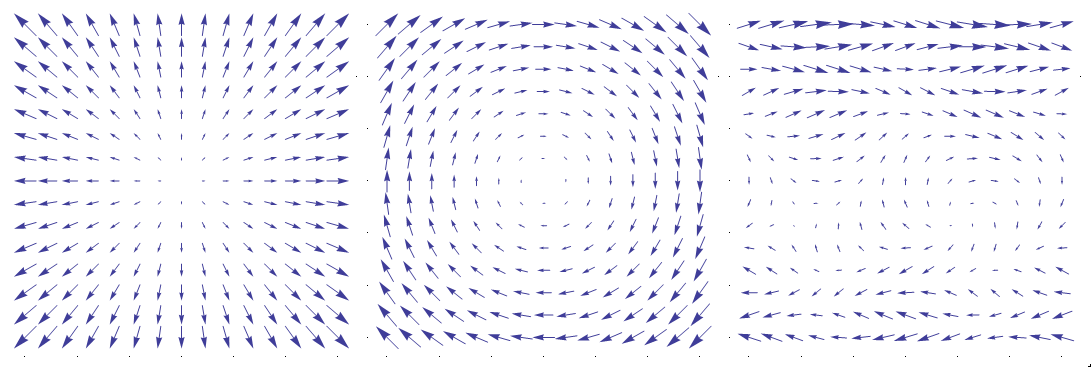
\includegraphics[scale= 0.4]{figures/vector_fields.png}}
  }

  \caption[Noise filterst]{Example of different types of vector fields.  \textbf{Left:} Divergent vector field. \textbf{Middle:} Rotational motion field. \textbf{Right:} Turbulent flow field with a significant amount of flow discontinuities.}
  \label{fig:vector_fields}
\end{figure*}

Divergence is a useful measure to analyze changes in velocity magnitude (i.e. acceleration). Additionally, divergence is a good indicator to identify potential errors in the computed optical flow field, since according to the smoothness assumption, the displacement field should vary slowly and violation of this fact can point out to problematic regions.  

An example of divergent vector field is given in Figure \ref{fig:vector_fields}. 

\subsubsection{Curl}
\label{curl}

\textit{Curl} is a vector operator which describes the rotation of a vector field. At a given point $\textbf{x}$ of the field $\textbf{F}(\textbf{x})$, it is represented as a vector, which characterizes the rotation at that point. The direction of the curl describes the rotations axis and the magnitude of the curl is the magnitude of rotation. 
For Cartesian coordinates, for a continuously differentiable vector field $\textbf{F}=(F_x,F_y,F_z)$ the curl is given by:
$$ \text{curl} \, \textbf{F} = \nabla \times \, \textbf{F} = \left( \frac{\partial F_z}{\partial y} - \frac{\partial F_y}{\partial z} \right) \textbf{i} + \left( \frac{\partial F_x}{\partial z} - \frac{\partial F_z}{\partial x} \right) \textbf{j} + \left(  \frac{\partial F_y}{\partial x} - \frac{\partial F_x}{\partial y} \right) \textbf{k},$$
where $\textbf{i}, \textbf{j}$ and $\textbf{k}$ are the unit vectors for x-,y-, and z-axes.
An example of rotational motion and corresponding vector field is given in Figure \ref{fig:vector_fields}. 


\subsubsection{Phase}
\label{phase}

Another useful measure to analyze the resulting flow field is a magnitude of the flow gradient. This measure is sensitive to any spatial variations of the motion field. 
For the 2-dimensional vector field $\textbf{F}=(F_x,F_y)$ the magnitude of the spatial gradient is given by:

$$ |\nabla_2 \textbf{F}|^2 =   \left( \frac{\partial F_x}{\partial x} \right)^2 + \left( \frac{\partial F_x}{\partial y} \right)^2 + \left( \frac{\partial F_y}{\partial x} \right)^2 + \left( \frac{\partial F_y}{\partial y} \right)^2 ,$$
where  $|f| = \sqrt{f^2_x + f^2_y}$ denotes the spatial magnitude and $\nabla_2 = (\partial_{x}, \partial_{y})$ the spatial gradient. For \textit{n}-dimensional vector field this expression can be generalized in a straightforward way by taking into account additional dimension.

It is important to note, that the given measure is equivalent to the formulation of homogeneous smoothness assumption \ref{homogeneous_smoothness} and can be used to measure discontinuities in the motion field. Figure \ref{fig:vector_fields} shows an example of a turbulent flow field with a large amount of flow discontinuities. 
      

%\subsection{Motion-Based Segmentation [TODO]}
%\label{motion_based_segmentation}
%
%
%\todo{Add content to this section}  
%Small overview for Motion based segmentation methods. 
%The general task for Motion based segmentation.
%Motion segmentation aims at decomposing a video in moving objects and background.
%
%%\comment{Which segmentation methods to show?}
%%\comment{IDEA: Present the adoption of popular segmentation methods (e.g. watershed or level sets) to vector data. Just show how to incorporate it.}
%
%\begin{figure*}[ht]
%  \centerline{
%    \mbox{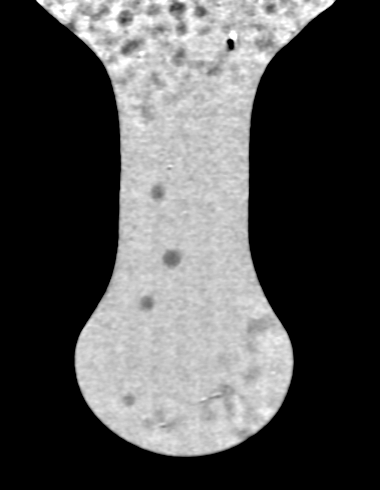
\includegraphics[scale= 0.28]{figures/seg_orig.png}}
%    \mbox{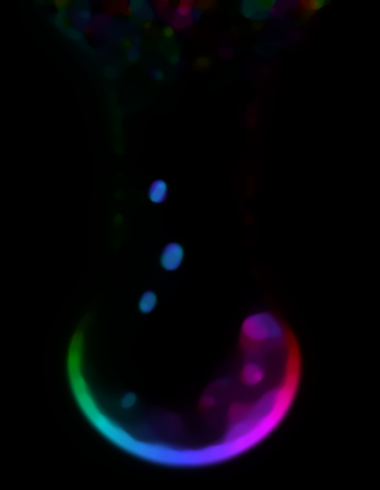
\includegraphics[scale= 0.28]{figures/seg_flow.png}}
%    \mbox{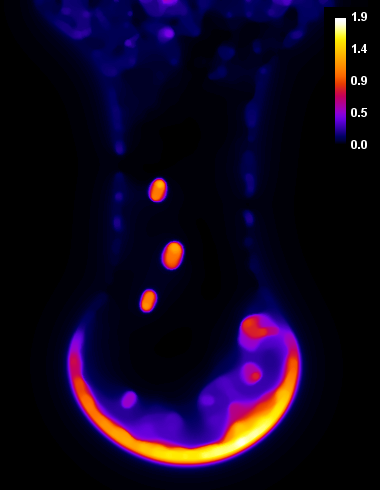
\includegraphics[scale= 0.28]{figures/seg_amp.png}}
%    \mbox{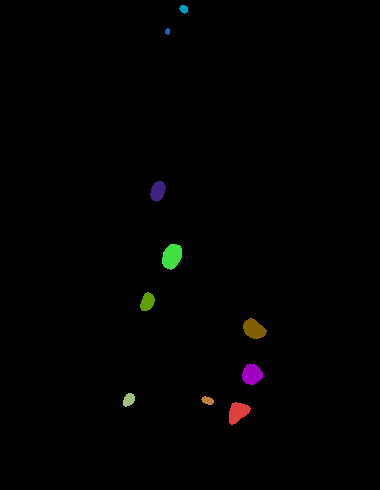
\includegraphics[scale= 0.28]{figures/seg_watershed.png}}
%  }
%
%  \caption[Noise filterst]{ \todo{Enlarge}. Examples of motion-based segmentation. \textbf{Left:} Input image of moving particles (dark spots). \textbf{Middle Left:} Flow field visualized using color-coding (color shows the direction, color brightness shows the magnitude). \textbf{Middle Right:} Segmentation using magnitude of the velocity field. \textbf{Right:} Motion-based segmentation using watershed segmentation on color-coded flow result. Both direction and flow magnitude are taken into account.}
%  \label{fig:motion_segmentation}
%\end{figure*}
%
%
%
%\begin{itemize}
%	  \item Using a flow-related measure as a label
%    \item Using contours?
%    \item Using colors + watershed
%\end{itemize}
       

\subsection{Object Tracking}
\label{tracking}


\textit{Object tracking} is an important task in the field of Computer Vision. It is used for a wide range of applications like video surveillance, human-computer
interaction, automated video analysis and autonomous vehicle navigation. For our application needs we are interested to track and analyses spatio-temporal evolution of various objects imaged by means of X-ray radiation: migrating cells, moving particles, changing structures, etc.


In the most general way, \textit{tracking} is a procedure of estimating the trajectory of an object within an 2D image plane (or 3D volume for tomographic data) as it changes its position over time.  Tracking involves three key steps: detection of moving objects, tracking of these objects within an image sequence, and analysis of their trajectories to learn about their dynamical behaviour.

In order to implement a tracking procedure one should consider a number of important aspects.
First, a suitable representation of the object should be defined. The next aspect is to choose an image feature which will be used to recognize the object. And, finally, an appropriate tracking strategy should be chosen. 

We describe these aspects step by step in the following sections. Note, that the object tracking is a well established and an extensive topic. Here we cover only those approaches which will be implemented within our data analysis framework (see Section \ref{data_analysis}), but additional methods could be  easily incorporated upon the need. For more details we refer the reader to the literature on tracking methods \cite{Yilmaz06, Trucco06}.  


\subsubsection{Object Representation}
\label{tracking_object_representation}

Here we describe common approaches to represent an object shape. In general, the choice of object representation determines the tracking algorithm. It is possible to distinguish the following representations:  
\begin{itemize}
   \item \textit{Points}. The simplest representation of an object is using a point. This point could be, for example, a geometrical center of the object (centroid) or some other characteristic feature. Moreover, complex objects can be represented by a set of points. In general,
a single point representation is well suited for tracking small objects (e.g. particles, cells).

  \item \textit{Primitive geometric shapes}. In this case an object is represented by a simple geometrical shape, such as a rectangle or an ellipse. The motion for such shapes is usually assumed to be described by affine transformations. Such geometrical shapes are useful to represent rigid object.
  
  \item \textit{Object contours}. Contour representation specify the boundary of an
object. This type of presentation is useful for tracking non-rigid objects. The contours are usually described using a special mathematical formulation, known as geodesic active contours or snakes \cite{Caselles95}. However, in the scope of our work we do not use this formulation. Instead, to represent a contour we use a multiple points, distributed on the edge of an object. This simplifies and reduces the number of tracking algorithms in our data analysis framework. 
    
\item \textit{Articulated shape or skeletal models}. Articulated objects are composed of several parts connected together with a joints mechanism. The relations between different parts are driven by a specified kinematic motion model (e.g. angles relations, stiffness). This representation is useful for tracking human or animal body parts. For our class of applications this model can also be useful, however in the current work we do not implement it.
\end{itemize}

As a base representation of objects we opt to choose a point representation, which is general and allows to define small objects with a single point, complex objects as a set of points and non-constant objects contours as a set of points distributed along the boundary of an object. Additionally, this allows us to have only one type of tracking algorithm (see Section \ref{object_tracking}).  


\subsubsection{Features for Tracking}
\label{tracking_features}

The crucial aspect is a choice of image features or object properties which are used for tracking. The requirements for such features are: they should be unique and provide a good description the object, they should also be robust to noise and other artifacts.
The commonly used visual features are:

\begin{itemize}
   \item \textit{Color}. The primary information about an object is its color or a brightness value. In the visual light imaging scenario the color is mainly determined by the illumination conditions of the scene and surface properties of the object (reflectance, diffusivity). In our case, the color represents the result of interaction of X-rays with a sample (e.g. attenuation of the upcoming radiation).  
   
   \item \textit{Edges}. Another characteristic property of an object is its boundaries.
   For this case an edge detection algorithm is used to identify the changes in image intensities, representing an object contour. There are several advantages for this feature. First, the edges are less sensitive to illumination changes. Second, they additionally provide orientational information. There are a number of easy to implement and accurate edge detection techniques available \cite{Canny86, Bowyer01}.   

	\item \textit{Optical Flow}. In this work the main feature used for tracking is a displacement vector computed by an optical flow algorithm. This vector is available for every pixel in the image (dense displacement field) and directly shows the new position of the given pixel on the next frame.

\item \textit{Texture}. Texture is feature which describes brightness variations on the surface or within an object. These variations might be caused by a pattern in the illumination or properties of the object itself. Usually, to quantify the texture a number of texture descriptors are used. Similar to an edge feature, texture based information is also robust with respect to illumination conditions and noise.
\end{itemize}

Depending on the application and available data, a combination of aforementioned features can be used. In the scope of this work we use an optical flow as the main source of information to perform tracking. In order to track contours of non-rigid or complex objects we additional may use the object edges to distribute a set of points for further tracking.  

\subsubsection{Object Tracking}
\label{object_tracking}

After the object representation and features of interest are chosen, the final step for the tracker algorithm is to estimate a trajectory of a moving object by locating its position in every frame of the image sequence.

The tracking procedure starts by detecting or identifying initial position of objects. In our work we mainly use the point representation for small objects and multiple points to represent complex objects. The distribution of points representing an object can be done manually by the user or distributed automatically. In case of automatic selection the points can be distributed randomly, using specified positions on a grid or according to image features discussed in Section \ref{tracking_features}.
 
The model which is selected to represent an object constraints the type of motion or deformation it can perform. For a point representation, the object motion is limited to translations. Tracking of an object represented by a single point is trivial, we just follow each point using a computed displacement vector.
A non-rigid object represented by multiple points defining its contour can move freely. In this case, by analyzing the new positions of the contour it is possible to learn about object's appearance. For a complex rigid object represented by multiple points we may introduce a number of motion constraints  \cite{Yilmaz06} to reconstruct its affine transformation. These constraints are schematically depicted in Figure \ref{fig:motion_constraints}.  
  
\begin{figure*}[ht]
  \centerline{
    \mbox{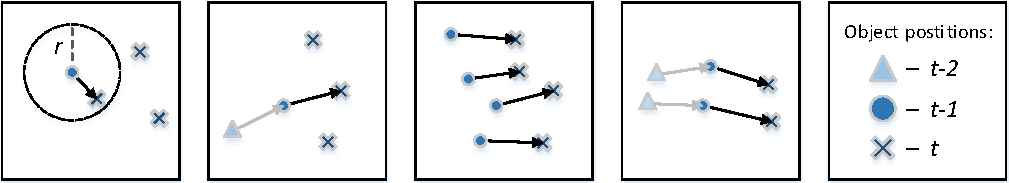
\includegraphics[width=0.98\textwidth]{figures/fig_38_p69.pdf}}
  }

  \caption[Noise filterst]{Different motion constraints. \textbf{Left:} Maximum velocity constrained to the radius $r$. \textbf{Middle Left:} Small velocity change constraint. \textbf{Middle Center:} Common motion. \textbf{Middle Right:} Rigidity constraints. Triangles denote object position at frame $t$-2, circles denote object position at frame $t$ - 1, and crosses  denote object position at frame $t$. \textbf{Right:} Scheme of pixel codes on different time frames. Image adopted from  \cite{Yilmaz06}.  }
  \label{fig:motion_constraints}
\end{figure*}

\begin{itemize}
	\item \textit{Maximum velocity} specifies an upper bound of the object velocity which it can undergo. This can be specified by a circular neighborhood around an object.
	\item \textit{Small velocity change} (temporal motion smoothness) assumes the direction and magnitude of the object's displacement does not change rapidly.
	\item \textit{Common motion} (spatial motion smoothness) constrains the displacements of nearby points within the object to be similar.
	\item \textit{Rigidity} assumes that objects are rigid, resulting that the distance between
any two points which belong to the object are unchanged after the .
\end{itemize}



%\subsection{Temporal Changes Detection}
%\label{temporal_changes_detection}
%
%Small overview for Temporal changes detection methods. The general task for Temporal changes detection.
%
%\subsubsection{Motion Compensated Difference}
%
%
%\begin{itemize}
%	\item Problem statement
%  \item Motivation
%  \item Limitations of Difference approach
%  \item The task for temporal changes detection method
%\end{itemize}


\subsection{Image Registration and Alignment}
\label{image_registration}


\textit{Image registration} is a process of aligning two or
more images of the same scene taken at different times,
from different views, or by different imaging techniques.  Registration is required in many fields, such as remote sensing, in medicine and in Computer Vision. An example of image registration of time-resolved tomographic data is shown in Figure \ref{fig:example_registration}.


%\begin{figure*}[ht]
%  \centerline{
%    \mbox{\includegraphicslabeledw[scale= 0.53]{figures/example_registration_a.png}{a}}
%    \mbox{\includegraphicslabeledw[scale= 0.53]{figures/example_registration_b.png}{b}}
%    \mbox{\includegraphicslabeledw[scale= 0.53]{figures/example_registration_c.png}{c}}
%    \mbox{\includegraphicslabeledw[scale= 0.53]{figures/example_registration_d.png}{d}}
%  }
%  
%  \vspace{3pt}
%  
%  \centerline{
%  	    \mbox{\includegraphicslabeledw[scale= 0.53]{figures/example_registration_e.png}{e}}
%  	    \mbox{\includegraphicslabeledw[scale= 0.53]{figures/example_registration_f.png}{f}}
%  	    \mbox{\includegraphicslabeledw[scale= 0.53]{figures/example_registration_g.png}{g}}
%  	    \mbox{\includegraphicslabeledw[scale= 0.53]{figures/example_registration_h.png}{h}}
%  }
%  \caption[Noise filterst]{Example of image registration using optical flow. Application: \textit{in-situ} analysis of void formation in flip-chip devices under electrical load. \textbf{(a)} First time frame of the image sequence. \textbf{(b)} Second frame. \textbf{(c)} Changes detection using image difference. Global sample movement cause a lot of falsely identified regions. \textbf{(d)} Image difference after image registration via optical flow. \textbf{(e-h)} After the image registration is performed, the tracking of voids evolution is possible . Colors show individual pores. Note, that all voids merge into a single one in the end of a sequence.}
%  \label{fig:example_registration}
%\end{figure*}

The task for image registration is to find the optimal  spatial and intensity transformations so the input images are matched. Image registration can be defined for two-dimensional images as a mapping between a target $I_1(x, y)$ and a reference $I_2(x,y)$ images, where $I(x,y)$ represents image intensity. Then, the mapping between these images can be expressed as following:
$$I_2(x,y) = g(I_1(f(x,y))),$$
where $f$ is a function which maps spatial coordinates $(x,y)$ into new locations $(x',y')$, such as $(x', y') = f(x,y)$ and $g$ is an intensity transformation.

Depending on the task and application field, it is possible to distinguish four classes of specific registration problems:
\begin{itemize}
\item \textit{Multimodal registration (different sensors)}: Registration of images of the same scene acquired using different imaging modalities. Example: Combine structural information form CT and functional brain activity from MRI imaging.

\item \textit{Template matching}: Match a reference pattern or a model with an image. Example: Registration of an image pattern with the model representation of the scene or atlas. 

\item \textit{Viewpoint registration (different views)}: Registration of a scene taken from different viewpoints. Example: Depth or shape reconstruction in Computer Vision.
 
\item \textit{Temporal registration}: Registration of images of the same scene taken at different time, under different imaging or physical conditions. Example: Detection and monitoring of changes in a scene, object or specimen.

\end{itemize}
In our work we mainly focus on the task of temporal registration to expose changes between subsequent images or perform image alignment of object position.

In general, image registration procedure consist of the four stages \cite{Zitova03}, which are similar to the common steps for object tracking (see Section \ref{tracking}):
\begin{itemize}

\item \textit{Feature detection}. Detection of salient and distinctive features such as objects, characteristic points, edges, contours, lines, corners, etc.
Such features can be placed manually or detected automatically.

\item  \textit{Feature matching}. Establish the correspondence between the features detected in the target and the reference image. To perform a matching procedure a number of spatial constraints and similarity measures are used.  

\item \textit{Transformation estimation}. A mapping between the target and the reference image is estimated according to established feature correspondences. 

\item \textit{Image resampling and transformation}. As a final step, the images are transformed towards each other using the estimated mapping function. For the mapping and resampling of intensity values an appropriate interpolation techniques is used.

\end{itemize}

All the differences within images in terms of pixel positions or intensity values due to the temporal changes or different acquisition conditions are referred as \textit{variations}.
It is important to distinguish between distortions and other variations. \textit{Distortions} are variations which are the source of misregistration.  Essentially it is the distortions between images which we would like to remove by registration procedure and reveal the changes of interest.
These distortions might be caused by the image noise, intensity changes, sample or detector movement or other unwanted effects \cite{Zitova03}.

Another important aspect, is to distinguish between global/local transformations and
global/local variations \cite{Brown92}.  A global transformation is described by the same mapping (e.g. single equation) and transforms the whole image. A local transformation maps different pixels according to their spatial localization.
The same holds for variations: some variations are due to the global process like camera misalignment or global sample movement, and some variations correspond to local differences.
To perform image registration it is crucial to take into account which kind of transformation is applied for which kind of variations. For instance, images may have local variations, but a global transformation can be used to align for a global change to assist in revealing small local changes.
We will cover these aspects in a Section \ref{image_registration_strategies} where we discuss different registration strategies. In the following section we describe all the relevant steps in image registration.



\subsubsection{Feature Detection}
\label{reg_feature_detection}

A crucial step for image registration is the selection of feature descriptors.
These features should be distinct, well distributed over the image and robust under different image artifacts (e.g. noise, brightness changes, artifacts).
It is possible to categorize most of the registration techniques according to feature detection approach in the following way: 
\\
\\
\textit{Area-based detection}. Area-based methods do not perform a separate feature detection step. Instead, these approaches perform the feature matching procedure directly, according to a specific similarity measure. We discuss these methods in the next Section \ref{reg_feature_matching}.
\\
\\
\textit{Feature-based detection}. This approach is based on the detection of salient and distinctive feature to perform image registration.  Whole range of characteristic information extracted from the image data can be used for this purpose. Such features might include: specific points, lines, corners, contours, texture, geometric shapes, etc. An important difference from the area-based methods is that this kind of features represent higher level of information and could correspond to a physical model of the scene. 
The procedure for feature detection is closely related to the similar task for object tracking discussed in Section \ref{tracking_features}, so the same set of feature detection tools might be used.






\subsubsection{Feature Matching}
\label{reg_feature_matching}

After the features are detected, the next step is to perform feature matching.
In this section we describe the methods which will be used in the scope of this work.
\\
\\
\textit{Area-based matching}. A first category of methods are called area-based methods.
Such methods are also known as \textit{correlation-like}
methods or template matching techniques \cite{Zitova03}. As we already mentioned in the previous Section \ref{reg_feature_detection}, these techniques combine the feature detection and matching procedures. The images are registered without characteristic data points, instead the whole image domain is used.

A classical approach for area-based registration is a \textit{cross-correlation}, which is a statistical method to find similarity between images.  For a template $T$ and target image $I$, the two-dimensional cross-correlation function estimates the similarity for each translation $(u,v)$ by:
$$ CC(u,v) = \sum_{x,y} T(x,y) I(x-u, y-v)). $$
If the best template match with a target image is given at a translation of $(i,j)$, the cross-correlation function will have its peak at $CC(i,j)$.

In the case, if the brightness of the image and template differs due to the varying  imaging conditions, the images can be first normalized. The normalized cross-correlation is then given by:
$$NCC(u,v) = \frac{\sum_{x,y} (T(x,y) - \mu_T) (I(x-u, y-v) - \mu_I)}{\sqrt{\sum_{x,y} (T(x,y) - \mu_T)^2 (I(x-u, y-v) - \mu_I)^2}}, $$
where $\mu_T$ and $\mu_I$ are mean values of the template $T$ and the image $I$ respectively.  

A similar, but more intuitive measure computes the sum of the squared differences (SSD) between a template and an image:
$$SSD(u,v) = \sum_{x,y} (T(x,y) - I(x-u, y-v))^2.$$

Another variant of area-based techniques is the so-called sequential similarity detection algorithm (SSDA). Which simply estimates an absolute differences between two images being matched.
This measure is given by:
$$SSDA(u,v) = \sum_{x,y} |T(x,y) - I(x-u, y-v)|.$$


Area-based techniques are useful for images which are misaligned by rigid transformation, preferably a translation. For more complex geometrical transformation (e.g. fast rotation) the model should be modified, which usually leads to a significant increase in computation load due to the extended search space. Another disadvantage of the area-based methods is a poor performance for noisy data or homogeneous images  without prominent details or structures. In these cases no distinct peak position could be estimated. For example, low-contrast data with noisy background or rotated spherical shape of the embryo with a lot of similar cell structures.
\\
\\
\textit{Feature-based matching}. For this class of techniques we assume that features in the reference and the target images are detected. The next step for feature-based matching is to establish correspondences between them.
There are a vast variety of methods to find such correspondences. We do not contemplate to describe  these algorithms. For the extensive overview of different matching techniques we refer the reader to surveys on image registration methods \cite{Brown92, Zitova03}.
One popular choice of feature-based matching technique is based on scale invariant feature transform (SIFT) \cite{Lowe04}. These methods show good performance for a broad range of transformation models between images. However, their use exceeds the scope of the current work.
In this work the feature correspondences for sparse or dense points are provided by the optical flow method and described by the computed displacement vector.


    
\subsubsection{Transformation Estimation}
\label{transform_estimation}

After correspondences between features are established
the mapping function which overlays the target image with the reference is constructed.
The key component of the registration procedure is a type and properties of a spatial transformation which implements such alignment.
 Since a wide range of transformation types may present within each image, the registration technique is restricted by a particular transformation model or parameters.
This transformation should remove only those image variations, which are the result of distortion and should be corrected. Other image difference (changes of interest) should remain unaffected be the registration procedure and will be used for further analysis. 

As we already disccussed in the Section \ref{image_registration}, transformation can be global and local.  The most common types of global transformations
are rigid, affine, projective, perspective
and polynomial. Within our work the most useful model is rigid transform, which we use to track  
objects that preserve their shape. Affine transformation is a more general type of transformation and includes translation, rotation, scaling, similarity transformation, reflection, shear mapping, and compositions of them.  Here we enlist three main transformation models:
\\
\\
\textit{Global mapping models}.
The most common global transformation is a rigid transform, which preserve all the geometric properties of the object. According to this transform each point $(x_1,y_1)$ of the first image is mapped to a point $(x_2, y_2)$ of the second image in the following way:

$${x_2 \choose y_2} = {t_x \choose t_y} + s
 \begin{pmatrix}
  \cos \theta & -\sin \theta  \\
  \sin \theta & \cos \theta \\
 \end{pmatrix} {x_1 \choose y_1},$$
where $t_x, t_y$ are translation vector components, $\theta$ is a rotation angle and $s$ is a scale factor. A rigid transform with a scaling factor could be useful to register datasets acquired with a cone beam geometry (with different object to beam distances). 


To estimate a transformation and its parameters global mapping methods based on point matching use a set of point correspondences. In this case, if a sufficient number of control points are provided, it is possible to derive the parameters of the transformation using two general methods: 
\begin{itemize}
\item \textit{Approximation} procedure estimates the overall transformation mapping in such a way, that matched points are aligned as close as possible. This is usually implemented with statistical optimization methods, e.g. least square approximation. The key assumption in this case, is that the matched points could be inaccurate, so the transformation should satisfy all the matches in an optimal way.
   
\item \textit{Interpolation} procedure finds the transformation mapping so the feature points match precisely and parameters in other locations are estimated using a special relation. This method is useful in the case if fewer, but more accurate matches are provided.    
\end{itemize}


\noindent \textit{Local mapping models}.
A significant drawback of global approaches is that these methods do not properly treat the transformations which are local. For this case a number of specific or modified registration methods are used. 
In this work we do not use this type of mapping models, so we opt to skip the description of such techniques.  For the overview of available methods the reader is referred to the works of \cite{Brown92, Zitova03}.
\\
\\
\textit{Elastic registration}.
A fundamentally different approach for the registration of images with
complex or local distortions is not to use
any parametric or global mapping functions.
The idea of \textit{elastic registration} was introduced in a seminal work of Bajcsy and Kovacic \cite{Bajcsy89}. In this method an image is represented as an elastic model (rubber-like) and transformations are described as deformation forces constrained by a stiffness or smoothness.
In the current work we use the results of optical flow to compute dense local displacements to perform elastic registration. In our case the data constancy assumption is serving as a metric for feature matching and smoothness constraint is a similar concept as in the case of elastic registration. Note, that the optical flow parameters should be chosen appropriately, depending on the task and amount of local variations to be corrected or revealed. 
   

\subsubsection{Image Resampling}

To apply a mapping transformation, which is computed in the previous steps, an appropriate image resampling and interpolation have to be employed. This transformation can be done in a forward and backward direction. The forward approach is hard to implement and could produce data outliers (hole or overlaps) due to multiple mapping or discretization problems. The backward registration is easier to implement and produce good results. 

There is a large number of choices for the interpolation procedure \cite{Parker83, Grevera98}. 
For our task we use a backward registration by means of bilinear interpolation described in Section \ref{compensation}. For the volumetric data we use a 3D variant of this transformation - trillinear interpolation.

\subsubsection{Image Registration Strategies}
\label{image_registration_strategies}


Here we summarize several strategies of image registration used in our data analysis framework:
\begin{itemize}
  \item \textit{Dense local registration via optical flow}. Features - dense pixels, matching procedure - dense optical flow,  transformation -  backward flow field interpolation. Application example: Register two images to obtain the maximum similarity. 
  \item \textit{Dense global registration via optical flow}. Global registration is achieved by using a coarse representation of the flow field or input images, i.e. using an increased smoothness constraints or presmoothing parameter. Features - dense pixels, matching procedure - optical flow, transformation - backward flow field interpolation. Application example: Register two images of the same scene to compensate for global elastic changes to reveal local changes. 
  \item \textit{Feature-based registration via optical flow}. Features - sparse set of landmarks, matching procedure - sparse optical flow correspondences, transformation - global transformation based  on approximation or interpolation (see Section \ref{transform_estimation}). Application example: align images based on automatically distributed landmarks.
  \item \textit{Global image registration with correlation-based technique}. Features - entire image (image-based matching) , matching procedure - correlation-based techniques (SSDA is a good choice, see Section \ref{reg_feature_matching} ).  Application example: align images to compensate for a global sample movement prior to the optical flow computation, which is sensitive for small changes.
\end{itemize}






%--------------------------------------------------------
%\section{[OPTIONAL] Visualization Methods}
%\label{visualization}
%--------------------------------------------------------

%The section gives a brief survey on existing visualization methods for time-varying data.
%The focus is on the practical use of the techniques for particular data analysis tasks.
%Examples of possible applications are also discussed.
%
%\subsection{Vector Field}
%
%[pages 1-2]
%
%\begin{figure*}[!ht]
%  \centerline{
%    \mbox{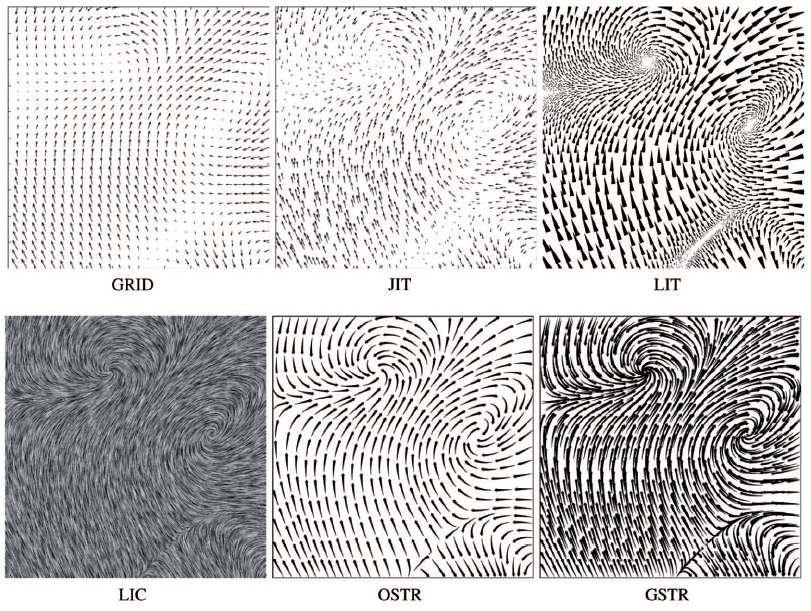
\includegraphics[scale= 0.55]{figures/vector_viz_types.png}}
%  }
%  \caption[]{\textbf{Left:} First frame of original image. \textbf{Middle:} With Gaussian noise.  \textbf{Right:} Parameter +2. Image source: \cite{Laidlaw05}}
%  \label{fig:lookup_tables}
%\end{figure*}
%
%\comment{Include information from vector fields visualization paper}
%        
%\begin{itemize}
%	\item Name
%  \item Description, Shows what?
%  \item Example image
%  \item Best usage examples
%\end{itemize}
%
%        
%\subsection{Scalar Field}
%
%[pages 0.5-1]
%
%\begin{itemize}
%	\item Name
%  \item Description, Shows what?
%  \item Example image
%  \item Best usage examples
%\end{itemize}
%
%
%Scalar field as a N-dimensional image can be repsesented in different color codes or Lookup tables (LUTs). 
%\change{From. Russ. Lookup tables (LUTs) can be implemented either in hardware or software. They use the original
%value as an index into a stored or precalculated table, which then provides the derived
%value. This process is fast enough that acquisition is not affected. LUTs
%are also used for displaying stored images, particularly to substitute colors for gray scale
%values to create pseudo-color displays.}
%
%\change{From. Russ.The use of color to encode richly multidimensional information must be distinguished from
%the very common use of false-color or pseudo-color to substitute colors for brightness in
%a monochrome image. Pseudo-color is used because of the limitation mentioned before in
%the visual ability to distinguish subtle differences in brightness. The use of color scales as a substitute for brightness values allows us to show and see small
%changes locally, and identify the same brightness values globally in an image. This should be
%a great benefit, since these are among the goals for imaging discussed below. Color might be used  to encode flow components, velocity, differently moving objects and other quantitative.
%These uses generally have little to do with the properties of the image and simply take advantage
%of the human ability to distinguish more colors than gray scale values.}
%An example of color coding using different LUTs is given in Figure \ref{fig:lookup_tables}.
%
%\begin{figure*}[!ht]
%  \centerline{
%    \mbox{\includegraphics[scale= 0.8]{figures/lookup_tables.png}}
%  }
%
%  \caption[Noise filterst]{\todo{Change image}. Taken from \cite{Russ11}. \textbf{Left:} First frame of original image. \textbf{Middle:} With Gaussian noise.  \textbf{Right:} Parameter +2.}
%  \label{fig:lookup_tables}
%\end{figure*}
%
%
%\subsection{Line Convolution}
%
%[pages 0.5-1]
%
%\begin{itemize}
%	\item Name
%  \item Description, Shows what?
%  \item Example image
%  \item Best usage examples
%\end{itemize}
%
%\subsection{Flow Streamlines}
%
%
%\begin{itemize}
%	\item Name
%  \item Description, Shows what?
%  \item Example image
%  \item Best usage examples
%\end{itemize}
%
%\subsection{Color Coding}
%
%Link: http://hci.iwr.uni-heidelberg.de/Static/correspondenceVisualization/
%
%To show:
%\begin{itemize}
%	\item 2D Bruhn colors
%	\item 2D Middl colors
%  	\item 3D RGB cube
%  	\item 3D projections: XY, YZ, XZ
%  	\item Simplified colors: 6, more
%\end{itemize}
%
%
%%\subsection{[OPTIONAL] Texture and Shape Coding}
%%
%%\comment{Find examples and code for texture-based coding}
%%
%%\begin{itemize}
%%	\item Name
%%  \item Description, Shows what?
%%  \item Example image
%%  \item Best usage examples
%%\end{itemize}
%
%\subsection{[OPTIONAL] Comparison of Visualization Methods}
%
%Comparison table of visualization methods. 
%Parameters to compare:
%\begin{itemize}
%	\item Direction
%    \item Magnitude
%    \item Density
%    \item Time evolution (like trajectories). Think about it. Check info in Vectors paper
%    \item 3D version
%\end{itemize}
%
%
%
%%--------------------------------------------------------
%\section {[OPTIONAL] Scientific software}
%%--------------------------------------------------------
%
%Section outline is here. \comment{Put the section here or to Appendix? Or skip completely?}
%
%\comment{Check Nature methods paper: Visualization of image data from cells to organisms}
%
%Description scheme:
%\begin{itemize}
%    \item Name
%    \item Short description
%    \item Features
%    \item Screenshot with visualization
%\end{itemize}
%    
%Comparison table in the end. TODO: Make a list of parameters to estimate.
%
%List of software to present:    
%\begin{itemize}
%	\item  ImageJ
%  \item  VTK
%  \item  Avizo/Amira
%  \item  Volume Studio MAX
%  \item  VisIt
%\end{itemize}

